\documentclass[../main.tex]{subfiles}
\begin{document}
\chapter{Lagrange's Theorem}
This very important theorem helps us to think about the orders of groups and subgroups.
We will first look at a simpler version of the theorem:
\begin{theorem}[Simple Lagrange's Theorem]
  If $H \leq G$  and $|G| < \infty$ then $|H| \mid |G|$.
\end{theorem}
The idea is to ``cut'' $G$ up into ``copies'' of $H$.
\section{Cosets}
These ``copies'' are called cosets of $H$ in $G$.
\begin{definition}[Left Coset]
  Let $H$ be a subgroup of $G$ and $g \in G$.
  The corresponding \textit{left coset} is:
  \[
    gH = \{gh : h \in H\} \subseteq G
  \]
\end{definition}
\begin{remark}[Notation]
  The set of all left cosets of $H$ in $G$ is $G / H$:
  \[
    G / H = \{gH : g \in G\}
  \]
\end{remark}
\begin{remark}
  We can also define \textit{right cosets} similarly:
  \[
    Hg = \{hg : h \in H\}
  \]
  Similarly, the set of right cosets of $H$ in $G$ is denoted by $H \setminus G$.
\end{remark}
\begin{lemma}
  If $H \leq G$, the left cosets partition $G$.
  That is:
  \begin{enumerate}
    \item The cosets of $H$ in $G$ cover $G$:
      \[
        G = \bigcup_{gH \in G / H} gH
      \]
    \item There is no ``overlap'' between cosets.
      That is for any $g_1H, g_2H \in G / H$:
      \[
        g_1H \cap g_2H \neq \emptyset \implies g1H = g_2H
      \]
  \end{enumerate}
\end{lemma}
\begin{proof}
  \begin{enumerate}
    \item For any $g \in G$, $g = g \cdot e \in gH$ so $\bigcup gH = G$.
    \item Suppose $g_1H \cap g_2H \neq \emptyset$.
      So there is $k \in g_1H \cap g_2H$ so for some $h_1, h_2 \in H$
      \begin{align*}
        k = g_1 h_1 &= g_2 h_2 \\
        g_1 &= g_2 (h_2 h^{-1}_{1})
      \end{align*}
      As $h_2 h^{-1}_{1} \in H$ we have that $g_1 \in g_2 H$.
      Furthermore, for any $h \in H$,
      \[
        g_1 h = g_2 ((h_2 h^{-1}_{1}) h) \in g_2 H
      \]
      This proves that $g_1H \subseteq g_2H$.
      By symmetry, $g_2 H \subseteq g_1 H$.
      Thus $g_1H = g_2H$.
  \end{enumerate}
\end{proof}
\begin{remark}[Note]
  $H$ itself is the coset $eH$.
\end{remark}
\begin{lemma}
  Let $H \leq G$.
  Then there is a bijection $H \to gH$ for any $g \in G$.
\end{lemma}
\begin{proof}
  The map $H \to gH$, $h \mapsto gh$ has inverse $gH \to H$, $gh \mapsto g^{-1}(gh) = h$.
\end{proof}
Since there is a bijection from the $H$ to any other coset, all cosets of $H$ over $G$ have the same size:
\begin{center}
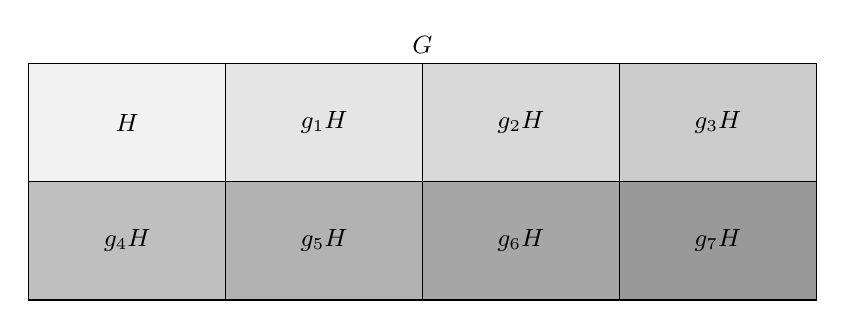
\begin{tikzpicture}[scale=1, every node/.style={font=\small}]
\def\ncols{4}
\def\nrows{2}
\def\w{2.5}
\def\h{1.5}

\draw[thick] (0,0) rectangle (\ncols*\w, \nrows*\h);
\node[above] at (\ncols*\w/2, \nrows*\h) {$G$};

\foreach \j in {1,0} {
  \foreach \i in {0,...,3} {
    \pgfmathtruncatemacro{\index}{\i + (1-\j)*\ncols}
    \pgfmathtruncatemacro{\shade}{10 + 10*\index}
    \filldraw[fill=gray!\shade, draw=black]
      (\i*\w, \j*\h) rectangle (\i*\w+\w, \j*\h+\h);
    \ifnum\index =0
      \node at (\i*\w+0.5*\w, \j*\h+0.5*\h) {$H$};
    \else
      \node at (\i*\w+0.5*\w, \j*\h+0.5*\h) {$g_{\index} H$};
    \fi
  }
}
\end{tikzpicture}
\end{center}

\begin{definition}[Index]
  The \textit{index} of a subgroup $H \leq G$ is:
  \[
    |G : H| = |G / H|
  \]
  That is, $|G : H|$ is the number of cosets of $H$ over $G$.
\end{definition}
\begin{remark}
  We could do a similar proof of the above using right cosets instead.
\end{remark}

\section{Lagrange's Theorem}
\begin{theorem}[Lagrange's Theorem]
  If $|G| < \infty$ then $|G| = |G : H| |H|$ for any $H \leq G$.
\end{theorem}
\begin{proof}
  Since left cosets partition $G$:
  \[
    |G| = \sum_{gH \in G / H} |gH| = \sum_{gH \in G / H} |H| = |G : H||H|
  \]
\end{proof}
\subsection{Corollaries of Lagrange's Theorem}
\begin{corollary}
  \label{orderDivCorollary}
  If $|G| < \infty$ and $g \in G$ then $|g| \mid |G|$.
\end{corollary}
\begin{proof}
  Recall that the order of $g$ is defined to be $|\langle g \rangle|$ and $|\langle g \rangle| \mid |G|$ by Lagrange's Theorem.
\end{proof}
\begin{corollary}
  If $|G| < \infty$ and $g \in G$ then $g^{|G|} = e$.
\end{corollary}
\begin{proof}
  From \cref{orderDivCorollary} we have that $|G| = k |g|$ for some $k \in \Z$, so:
  \[
    g^{|G|} = (g^{|g|})^{k} = e^{k} = e
  \]
\end{proof}
\begin{corollary}
  If $|G|$ is prime them $G$ is cyclic and any element $g \neq e$ generates $G$.
\end{corollary}
\begin{proof}
  Choose any $g \neq e$.
  From Lagrange's Theorem we know that $|g| \mid |G|$.
  Since $|G|$ is prime, either $|g| = 1$ or $|g| = |G|$.
  But $g \neq e$ so $|g| \neq 1$, thus $|g| = |G|$.
  This means that the cyclic group generated by $g$ is the same size as $G$ and is a subgroup of $G$.
  Therefore $G = \langle g \rangle$.
  So $g$ generates $G$ and $G$ is cyclic.
\end{proof}
\section{Application to Number Theory*}
\nonexaminable
Lagrange's Theorem implies an important result in Numbers \& Sets.
\begin{definition}[Euler Totient Function]
  \[
    \varphi(n) = |\{x \in \Z_n : \gcd(x, n) = 1\}|
  \]
  That is, $\varphi(n)$ counts the number of positive integers less than $n$ that are coprime to $n$.
\end{definition}
\begin{remark}[Notation]
  Let $\times_n$ denote multiplication mod $n$.
  This is associative and has identity $1$.
\end{remark}
\end{document}
